\documentclass{ba-kecs}
\usepackage{graphicx,, url}
\usepackage[numbers]{natbib}

\title{Turtlebot SLAM }

\author{Maurice Hermans, Lukas Kang, Michael Norget, Thomas Nowicki, Oliver Trinnes}

\begin{document}

\maketitle

\begin{abstract}
This article accompanies the research project ``TurtleBot SLAM'' from the Master ``Artificial Intelligence'' of Maastricht University.
\end{abstract}

\section{Introduction}
Nowadays a lot of tasks are performed by mobile robots, for example transportation, search and rescue and automated vacuum cleaning. To efficiently perform these tasks the robot needs a map of its environment. Sometimes the data about the environment is already available and using for example GPS the robot can locate itself, making the solving of the task at hand easier. But for other tasks the robot should only rely on internal sensors and make its own map of the environment.

The acquisition of these maps has been a major research focus in the robotics community the last decades. Building or learning these maps under the uncertainty of position and the accuracy of measurements is often referred to as the Simultaneous Localization And Mapping (SLAM) problem. A large variety of solutions is available to the SLAM problem, these approaches can be classified as either filtering or smoothing.

Filtering approaches model the problem as an on-line state estimation where the state of the system consists in the current robot position and the map. New measurements augment and refine the estimate as they come available. Due to their incremental nature these filtering approaches are usually referred to as on-line SLAM methods. The other type of approach estimates the full trajectory from the full set of measurements. These approaches address the so called full SLAM problem and they typically rely on least-square error minimization techniques.

An intuitive way to formulate the SLAM problem is to cast it as a pose graph optimization problem. Where the nodes represent robot poses or landmarks and in which the edges encode sensor measurements that constraint the connected poses. Once such a graph is constructed the method will try to find a configuration of the nodes that is maximally consistent with the measurements.

The rest of this paper is structured as follow. Section 2 will provide the reader with the necessary background information on this topic.

\begin{figure}[htbp]
	\centering
		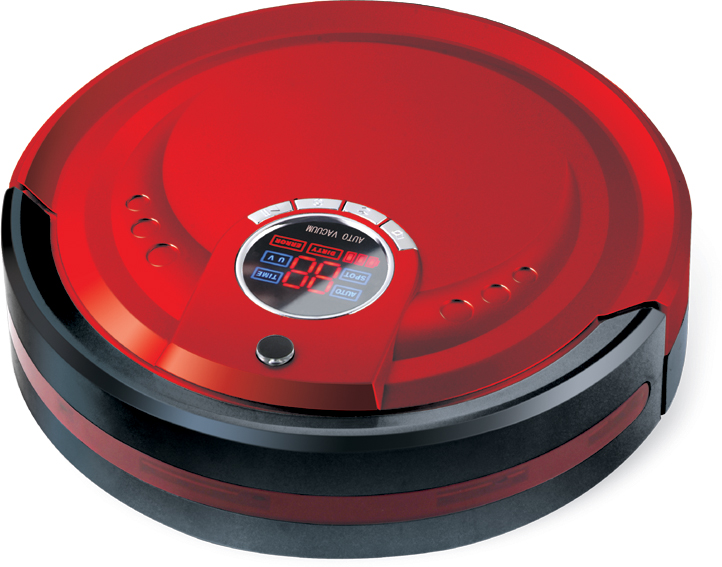
\includegraphics[width=0.50\textwidth]{vacuum_cleaner.jpg}
	\caption{Automated vacuum cleaner}
	\label{fig:vacuum_cleaner}
\end{figure}

\subsection{Problem Statement}
The focus of this paper is SLAM, more specifically GraphSLAM and how it is used to construct a map of an unknown environment. GraphSLAM returns as a result the optimal graph representing the path the robot has explored. There is also the need for exploration to map the still unseen areas of the space where the robot is located. Since the goal of the robot in this paper is to map the entire area where it has been placed. The data returned by the GraphSLAM algorithm is turned into a occupancy grid map and then used for the autonomous exploration. Each time the robot takes another sensor measurement of its surroundings a node is added to the data in the GraphSLAM algorithm, all the obstacles detected in a measurement are as reference points to optimize the graph. The algorithm is tested in a robot simulator named STAGE with a provided map.

\section{State of the art}
\subsection{ROS}
ROS (Robot Operating System) \cite{Quigley}, is the framework used in this paper to program the robots and it provides an environment to run simulations for the implemented algorithm. As described by Quigley et al. \cite{Quigley}, writing software for robots is difficult since there are so many possible hardware setups which makes code reuse nontrivial. Adding to this problem of hardware setups is the amount of code needed as it must contain a deep stack starting from driver-level software going up through perception, abstract reasoning and beyond. Since the required expertise is well beyond the capabilities of a single researcher, robotics software architectures must also support large scale software integration efforts.

To deal with the above mentioned problems many robotics researchers have created a wide variety of frameworks to deal with this complexity and facilitate them with the needs for their own research. This resulted in the many robotic software systems currently used by academia and industry \cite{Kramer}. Each of these frameworks was designed for a specific purpose, perhaps the available frameworks did not meet the requirements this researcher had or the emphasis was on the wrong aspects according to the researcher.

The ROS framework used in this paper is also the product of trade-offs and prioritizations. The emphasis of this framework is on large-scale integrative robotics research, making it useful in a wide variety of situations.

\subsection{TurtleBot}
The robots on which the algorithm from this paper will be tested are called TurtleBots, see figure \ref{fig:turtlebot}, the simulator will also mimic these robots. The TurtleBot is a low-cost, customizable, personal robot kit with open-source software. As a base iRobot Create is used (A) which holds a battery pack and 150 degrees/second Single Axis Gyro. The model shown in figure  \ref{fig:turtlebot} uses a Microsoft Kinect as sensor (B), the one used in this paper uses a laser range sensor, and a laptop (C) to run all the processes. The robot can also be customized using the mounting hardware (D). The robot runs on an open-source SDK based on ROS which integrates all the software needed to get the TurtleBot running and already includes some advanced capabilities like mapping and navigation.

\begin{figure}[htbp]
	\centering
		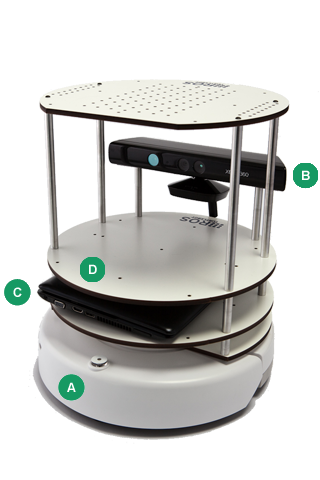
\includegraphics[width=0.50\textwidth]{turtlebot.png}
	\caption{A TurtleBot}
	\label{fig:turtlebot}
\end{figure}

\subsubsection{TurtleBot simulator}
To help with development a simulator is used to simulate the TurtleBots, the one used in this paper is called Stage. In stage it is possible to load layouts of rooms, called worlds, to simulate the robot being placed there. Once a world is loaded into stage one can drive around using manual or autonomous navigation. In stage it is possible to visualize the data the robot uses, for example the laser scans it is measuring or the path it has traveled. Then there is another tool to visualize the output of the algorithm the robot is performing, the 3D visualization tool rviz. This tool helps to evaluate and validate the output returned when performing the GraphSLAM algorithm.

\subsection{Exploration}
Many robots can navigate using maps provided to them, usually the mapping is done by humans before the robot is send to perform its task, this however limits the robot in its ability to navigate in unknown environments. The robots discussed in this paper however do not know anything of their environment at the start and need to build their own map. Thats why robots should be able to explore their environment, which we will define as the act of moving through an unknown environment while building a map that will be used for subsequent navigation. A good exploration strategy is one that generates a (nearly) complete map in the shortest amount of time.

Since the robot does not know anything about its environment the central idea is that it should move to where it would gain as much information as possible. This target should be extracted from the information the robot has obtained so far. Initially the robot knowns nothing except what is measures with its sensors. The map the robot creates should be as complete as possible and build as quickly as possible.

To achieve this the robot makes use of the idea of frontier-based exploration, first introduced by Yamauchi \cite{Yamauchi}. Frontiers are regions on the boundaries between open explored and unexplored space. When a robot moves to a frontier it will take measurements of unexplored space and add this new information to its map. As a result the explored region on the map expands and new frontiers are added to the map. By constantly moving to frontiers the robot can keep expanding its knowledge about the environment. Note that when the robot detects an obstacle there will be no frontiers behind them since it is no region separating open explored from unexplored space.

The performance of the exploration is then not only depending on the strategy the robot uses to select frontiers to explore but also on how to incorporate the new information into the map. This is a challenge since all the new information obtained is effected by noise, not only on the sensor measurements but also on the odometry data used to incorporate newly obtained information.

\subsection{SLAM}
To navigate through an unknown environment a robot needs to be able to build a map of the environment and simultaneously be able to localize itself within this map. This is called Simultaneous Localization And Mapping (SLAM). It basically means that the robot should be able to learn the map under pose uncertainty.

A large variety of solutions is available to the SLAM problem. These approaches can be classified into two categories, namely filtering and smoothing. 

The filtering approaches make a state estimation where the state of the system are stored in the current position and the map. New measurements are incorporated as they become available. In this category fall popular techniques like Kalman filters, particle filters, or information filters.

Conversely, the smoothing approaches keep using all measurements to estimate the entire trajectory the robot has traveled.

\subsubsection{GraphSLAM}
An intuitive way to address the SLAM problem is to pose it as a graph optimization problem. A graph will be constructed where the nodes represent robot poses or landmarks and where edges correspond to measurements that constraint the connecting nodes. Note that constraints can be contradictory because of the noise on the measurements. Once a graph is constructed the algorithm will try to find a configuration of the nodes that is maximally consistent with the measurements.

\section{Implementation}
\subsection{Wavefront frontier detection}
\subsection{GraphSLAM}
\subsubsection{Scan matching}
\subsection{Mapping}
Figure \ref{fig:random_map} shows a partial map created by the ROS gmapping package.
\begin{figure}[htbp]
	\centering
		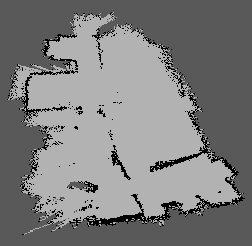
\includegraphics[width=0.50\textwidth]{random_map.png}
	\caption{A partial map}
	\label{fig:random_map}
\end{figure}

\section{Experiments and Results}
\subsubsection{Benchmarks}

\section{Discussion}
\subsubsection{Future research}

\section{Conclusion}

\bibliography{references}
\nocite{*}
\onecolumn
\appendix

\end{document}
